%D�finir le format du document: papier, taille de police, type de document, etc.
\documentclass[a4paper, 11pt]{article}

%%%%%%%%% Packages externes utilis�s %%%%%%%%%%%%%%%%%%%
\usepackage[french]{babel}
\usepackage[latin1]{inputenc}
\usepackage[T1]{fontenc}
\usepackage{verbatim}
\usepackage{graphicx}
\usepackage{epstopdf}
\usepackage{amsmath}
\usepackage{amssymb}
\usepackage{macro}
\usepackage{algorithm}
\usepackage{algorithmic}
\usepackage{xcolor}
\usepackage{textcomp}
\usepackage{listings}
\lstset{
language=C,
basicstyle=\normalsize, % ou �a==> basicstyle=\scriptsize,
upquote=true,
aboveskip={1.5\baselineskip},
columns=fullflexible,
showstringspaces=false,
extendedchars=true,
breaklines=true,
showtabs=false,
showspaces=false,
showstringspaces=false,
identifierstyle=\ttfamily,
keywordstyle=\color[rgb]{0,0,1},
commentstyle=\color[rgb]{0.133,0.545,0.133},
stringstyle=\color[rgb]{0.627,0.126,0.941},
}
%\usepackage{algorithm2e}


%La mise en page du rapport, NE PAS MODIFIER.
\usepackage{geometry}
 \geometry{
 a4paper,
 left=20mm,
 right=20mm,
 top=20mm,
 bottom=20mm,
 }

%%%%%%%%% Le corps du document entre begin et end %%%%%%%%%%%%%%%%%%%
\begin{document}

\section*{Mavlink communication}
\label{sec:mavlink_communication}

\noindent In this document, we will explain how mavlink communication works in an UDP program.


\subsection*{Initialization}
\label{sec:initialization}

\paragraph{} Firts of all you need to know how to initialize UDP connection for listen and send packets.

\paragraph{-Initialize listening} This first step is the more simple, you only have to initialize a listening socket on the port 14550 (port where the controller send informations) and bind it.

\begin{lstlisting}
struct sockaddr_in locAddr;
int sock = socket(PF_INET, SOCK_DGRAM, IPPROTO_UDP);

locAddr.sin_family = AF_INET;
locAddr.sin_addr.s_addr = INADDR_ANY;
locAddr.sin_port = htons(14550);
memset (&locAddr.sin_zero, 0, sizeof(locAddr.sin_zero));

if (-1 == bind(sock,(struct sockaddr *)&locAddr, sizeof(struct sockaddr))){
	perror("error bind failed");
	close(sock);
    	return -1;
}
\end{lstlisting}

\paragraph{-Initialize sending} This step is more complicated because the target port always changes. The solution that we have found is to listen, with the listening socket initialized previously, all incoming messages and stop when we receive one from the target IP : 10.1.1.1 (adress of the controller). Thus we get the target port and we can initialize the sending socket.

\begin{lstlisting}
struct sockaddr_in targetAddr;
targetAddr.sin_family = AF_INET;
targetAddr.sin_addr.s_addr = inet_addr("10.1.1.1");
targetAddr.sin_port = possibleTarget.sin_port;
memset (&targetAddr.sin_zero, 0, sizeof(targetAddr.sin_zero));
\end{lstlisting}


\subsection*{Receive mavlink by UDP}
\label{sec:receive}

\paragraph{-Buffer} First of all you need intialize a buffer that you fill block of memory at each use with "memset" :

\begin{lstlisting}
#define BUFFER_LENGTH 2041
...
uint8_t buf[BUFFER_LENGTH];
...
memset(buf, 0, BUFFER_LENGTH);
\end{lstlisting}

\paragraph{-Receiving} After that, you receive bytes with de function "recvfrom".

\begin{lstlisting}
recsize = recvfrom(sock, (void *)buf, BUFFER_LENGTH, 0, (struct sockaddr *)&targetAddr, &fromlen);	
\end{lstlisting}

\paragraph{-Parsing} Then you parse it in order to convert it in a mavlink message, thus you can interpret this message.

\begin{lstlisting}
if (mavlink_parse_char(chan, buf[i], &msg, &status)){
	printf("\nReceived packet: SYS: %d, COMP: %d, LEN: %d, MSG ID: %d\n\n", msg.sysid, msg.compid, msg.len, msg.msgid);
}
\end{lstlisting}


\subsection*{Send mavlink by UDP}
\label{sec:send}

\paragraph{-Buffer} First of all you need intialize a buffer that you fill block of memory at each use with "memset" like before :

\begin{lstlisting}
#define BUFFER_LENGTH 2041
...
uint8_t buf[BUFFER_LENGTH];
...
memset(buf, 0, BUFFER_LENGTH);
\end{lstlisting}

\paragraph{-Packing} Second step is to "pack" the mavlink message with the "pack function". There are numerous type of  "pack function" and for various uses, we will dwell on these different types later, for the moment we will use the basic message "heartbeat" which is a frequent message to give "sign of life" of a device.

\begin{lstlisting}
mavlink_msg_heartbeat_pack(255,0,&msg,MAV_TYPE_GCS,MAV_AUTOPILOT_ARDUPILOTMEGA,0xc0,0x0,MAV_STATE_ACTIVE);
\end{lstlisting}

\paragraph{-Converting} After being pack, we put the mavlink message in the buffer with the function "mavlink\_msg\_to\_send\_buffer".

\begin{lstlisting}
len = mavlink_msg_to_send_buffer(buf, &msg);
\end{lstlisting}

\paragraph{-Sending} To finish, send the buffer with the function "sendto".

\begin{lstlisting}
bytes_sent = sendto(sock, buf, len, 0, (struct sockaddr*)&targetAddr, sizeof(struct sockaddr_in));
\end{lstlisting}


\subsection*{Decode mavlink message}
\label{sec:decode}

\paragraph{} In the part \ref{sec:receive} we have seen how to get a mavlink message. Now we are going see how to decode it and how to diplay his informations.

\paragraph{-Identified} First of all you have to know that each mavlink message have a message id that indicate the type of message encapsulated. Thus we only have to compare the field "msgid" of the message with the macro constant
of a type. To have more informations about tram's construction and about the different types, we recommend you to see the documents mavlink-devguide.pdf and mavlink\_protocol.pdf.

\begin{lstlisting}
if(msg.msgid == MAVLINK_MSG_ID_SYS_STATUS)	//If the message is of type SYS_STATUS
\end{lstlisting}

\paragraph{-Decoding} When you have identified the type, you need to create a variable of this type in order to call the right decode function to put information into the variable. To find the type and the fonction's name you have to go in the corresponding file of the library.

\begin{lstlisting}
mavlink_sys_status_t sys_status;
mavlink_msg_sys_status_decode(&msg, &sys_status);
\end{lstlisting}

\paragraph{-Displaying} To finish, if you want to see the data contents into the variable, you simply have to print  fields of the structure. In the same way, to know their name, you have to go in the file of the corresponding type. 

\begin{lstlisting}
printf("SYS_STATUS :\nOnboard_control_sensors_present : %d, Onboard_control_sensors_enabled : %d, Onboard_control_sensors_health : %d, Load : %d, Voltage_battery : %d, Current_battery : %d, Drop_rate_comm : %d, Errors_comm : %d, Errors_count1 : %d, Errors_count2 : %d, Errors_count3 : %d, Errors_count4 : %d, Battery_remaining : %d\n\n", sys_status.onboard_control_sensors_present, sys_status.onboard_control_sensors_enabled, sys_status.onboard_control_sensors_health, sys_status.load, sys_status.voltage_battery, sys_status.current_battery, sys_status.drop_rate_comm, sys_status.errors_comm, sys_status.errors_count1, sys_status.errors_count2, sys_status.errors_count3, sys_status.errors_count4, sys_status.battery_remaining);
\end{lstlisting}


\subsection*{Send mavlink order}
\label{sec:order}

\paragraph{} As we have seen in the part \ref{sec:send} we have to call a "pack function" in order to send mavlink message. Now we are going see what packs can be used to send an order to drone.

\paragraph{-Set mode} To request to change the flight mode you need to call the function "mavlink\_msg\_set\_mode\_pack". The first parameter is the system id of the source (255 because we simulate a QGC), the second one is the component id of the source, the third is the mavlink message that we want to pack, the fourth is system id of the target (1 for all vehicle) and the others the type of flight mode choice.

\begin{lstlisting}
mavlink_msg_set_mode_pack(255, 0, &msg, 1, MAV_MODE_MANUAL_ARMED+MAV_MODE_FLAG_CUSTOM_MODE_ENABLED, COPTER_MODE_ALT_HOLD); 
\end{lstlisting}

\paragraph{-Command long} For many orders the "pack function" which is called is "mavlink\_msg\_command\_long\_pack". His four first parameters are the same than before, after that we have the component id of the target and then the type of command. The rest of the parameters depends of the command. Thus with this kind of function we can send the order to arm the drone like below :

\begin{lstlisting}
mavlink_msg_command_long_pack(255, 0, &msg, 1, 0, MAV_CMD_COMPONENT_ARM_DISARM, 0, 1, 0, 0, 0, 0, 0, 0);
\end{lstlisting}


\subsection*{Send mavlink mission}
\label{sec:mission}

\noindent In this section we will describe how a mission is made and how to prepare and send one to the drone.


\paragraph{-Mission count} First of all, you have to send a MAVLINK\_MSG\_ID\_MISSION\_COUNT. The contents of the different fields of the message are : 

\begin{itemize}
\item count = (2 or 4 or ...), represents the number of mission items in the sequence
\item target\_system = 1 (0x01), the ID of the target system.
\item target\_component = 190 (0xbe), the ID of the target component
\end{itemize}

\begin{figure}[H]
	\centering
		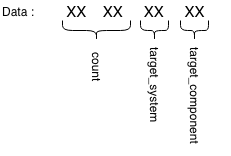
\includegraphics[scale=0.6]{./images/MAVLINK_MSG_ID_MISSION_COUNT.png}
		\caption{Show how a mission count frame is built}
	\label{fig:MISSION_COUNT}
\end{figure}

\noindent Example of function call for packing a mission count message :

\begin{lstlisting}
mavlink_msg_mission_count_pack(255, 0, &msg, 1, 190, 2);	//MISSION_COUNT
\end{lstlisting}


\paragraph{-Mission item} Next, you send some MAVLINK\_MSG\_ID\_MISSION\_ITEM depending on the mission you want to perform. The contents of the different fields of the message are :
\begin{itemize}
\item param1 = depends on the command, see in MAV\_CMD enum.
\item param2 = depends on the command, see in MAV\_CMD enum.
\item param3 = depends on the command, see in MAV\_CMD enum.
\item param4 = depends on the command, see in MAV\_CMD enum.
\item x = depends on the command, local: X coordinate, global: latitude.
\item y = depends on the command, local: Y coordinate, global: longitude.
\item z = depends on the command, local: Z coordinate, global: altitude (relative or absolute, depending on frame).
\item seq = sequence (0, 1, 2, 3, ...).
\item command = MAV\_CMD\_NAV\_WAYPOINT (0x0010 = 16) or MAV\_CMD\_NAV\_TAKEOFF (0x0016 = 22) or MAV\_CMD\_DO\_CHANGE\_SPEED (0x00b2 = 178) or ...
\item target\_system = 1 (0x01), the ID of the target system.
\item target\_component = 190 (0xbe), the ID of the target component.
\item frame = MAV\_FRAME\_GLOBAL (0x0000 = 0) or MAV\_FRAME\_GLOBAL\_RELATIVE\_ALT (0x0003 = 3) or MAV\_FRAME\_MISSION (0x0002 = 2) or ..., see more in MAV\_FRAME enum. The coordinate system of the waypoint.
\item current = 1 for the first item, 0 for the following items.
\item autocontinue = 1, autocontinue to next waypoint.
\end{itemize}

\begin{figure}[H]
	\centering
		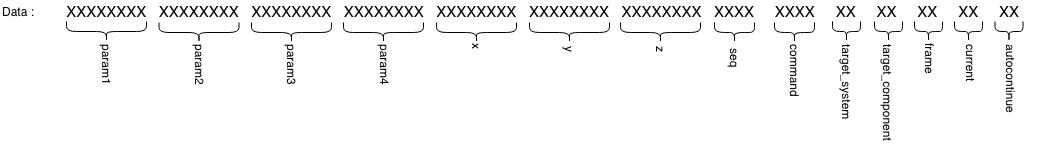
\includegraphics[scale=0.5]{./images/MAVLINK_MSG_ID_MISSION_ITEM.png}
		\caption{Show how a mission item frame is built}
	\label{fig:MISSION_ITEM}
\end{figure}

\noindent Examples of function call for packing a mission item message :

\begin{lstlisting}
mavlink_msg_mission_item_pack(255, 0, &msg, 1, 190, 0, MAV_FRAME_GLOBAL, MAV_CMD_NAV_WAYPOINT, 1, 1, 0, 0, 0, 0, gps_raw_int.lat, gps_raw_int.lon, gps_raw_int.alt);	//MISSION ITEM WAYPOINT
...
mavlink_msg_mission_item_pack(255, 0, &msg, 1, 190, 1, MAV_FRAME_GLOBAL_RELATIVE_ALT, MAV_CMD_NAV_TAKEOFF, 0, 1, 15, 0, 0, 0, 0, 0, 1);	//MISSION ITEM TAKEOFF 1m
\end{lstlisting}


\paragraph{-Set mode} Then, you send a MAVLINK\_MSG\_ID\_SET\_MODE in order to put the drone in guided mode. The contents of the different fields of the message are :
\begin{itemize}
\item target\_system = 1, the ID of the target system.
\item custom\_mode = COPTER\_MODE\_GUIDED (0x0004 = 4) or COPTER\_MODE\_LAND (0x0009 = 9), see more in COPTER\_MODE enum.
\item base\_mode = MAV\_MODE\_GUIDED\_DISARMED+MAV\_MODE\_FLAG\_CUSTOM\_MODE\_ENABLED (0x59 = 89) or MAV\_MODE\_GUIDED\_ARMED+MAV\_MODE\_FLAG\_CUSTOM\_MODE\_ENABLED (OxD9 = 217), see more in MAV\_MODE and MODE\_FLAG enum.
\end{itemize}

\begin{figure}[H]
	\centering
		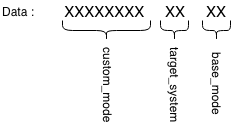
\includegraphics[scale=0.5]{./images/MAVLINK_MSG_ID_SET_MODE.png}
		\caption{Show how a set mode frame is built}
	\label{fig:SET_MODE}
\end{figure}

\noindent Example of function call for packing a set mode message :

\begin{lstlisting}
mavlink_msg_set_mode_pack(255, 0, &msg, 1, MAV_MODE_GUIDED_DISARMED+MAV_MODE_FLAG_CUSTOM_MODE_ENABLED, COPTER_MODE_GUIDED); // Request change flight mode
\end{lstlisting}


\paragraph{-Command long}  Then, you send 2 MAVLINK\_MSG\_ID\_COMMAND\_LONG in order to arm and to start the mission. The contents of the different fields of the message are :
\begin{itemize}
\item param1 = 1 or 0, depends on the command, see in MAV\_CMD enum
\item param2 = depends on the command, see in MAV\_CMD enum
\item param3 = depends on the command, see in MAV\_CMD enum
\item param4 = depends on the command, see in MAV\_CMD enum
\item param5 = depends on the command, see in MAV\_CMD enum
\item param6 = depends on the command, see in MAV\_CMD enum
\item param7 = depends on the command, see in MAV\_CMD enum
\item command = MAV\_CMD\_COMPONENT\_ARM\_DISARM (0x0190 = 400) or MAV\_CMD\_MISSION\_START (0x012C = 300)
\item target\_system = 1, the ID of the target system.
\item target\_component = 1, the ID of the target component.
\item confirmation = 0 : first transmission of this command, 1-255 : confirmation transmissions.
\end{itemize}

\begin{figure}[H]
	\centering
		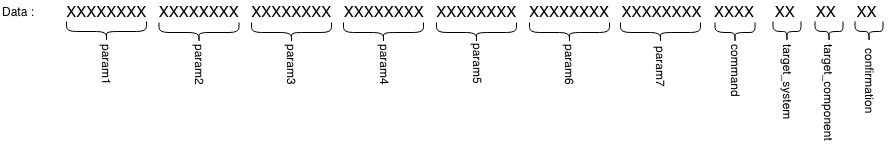
\includegraphics[scale=0.5]{./images/MAVLINK_MSG_ID_COMMAND_LONG.png}
		\caption{Show how a command long frame is built}
	\label{fig:COMMAND_LONG}
\end{figure}

\noindent Example of function call for packing a command long message :

\begin{lstlisting}
mavlink_msg_command_long_pack(255, 0, &msg, 1, 1, MAV_CMD_COMPONENT_ARM_DISARM, 0, 1, 0, 0, 0, 0, 0, 0);	//Request arm motors
...
mavlink_msg_command_long_pack(255, 0, &msg, 1, 1, MAV_CMD_MISSION_START, 0, 0, 0, 0, 0, 0, 0, 0);	//Request start mission
\end{lstlisting}


\subsection*{Sources}
\label{sec:Sources}

\begin{itemize}
\item Mavlink library version 1 in c : https://github.com/mavlink/c\_library\_v1
\item Small example using the library in c : https://mavlink.io/en/examples/c\_udp.html
\item IP adress communication : https://unix.stackexchange.com/questions/320640/3dr-solo-drone-wifi-communication
\item Port communication : https://github.com/PX4/Devguide/issues/357
\item Message ID macro and values : https://groups.google.com/forum/\#!topic/mavlink/1zgHUM67E-
A
\end{itemize}




\end{document}
